\documentclass[a4paper]{article}

\usepackage{tikz}
\usetikzlibrary{bayesnet}
\begin{document}

% node:       \node[type](name){caption}
% factor:     \factor[options]{name}{caption}{in}{out}
% plate:      \plate[options]{name}{fitlist}{caption}
% edge:       \edge[options]{inputs}{outputs}
% factoredge: \factoredge[options]{inputs}{factor}{outputs}

\begin{figure}[ht]
  \begin{center}

    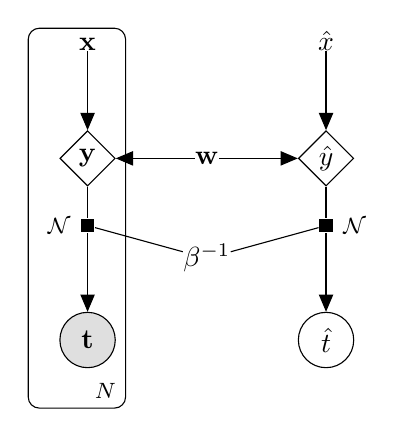
\begin{tikzpicture}

      % Define nodes
	  \node[const]                             (x) {$\mathbf{x}$};
	  \node[det, below=of x]                   (y) {$\mathbf{y}$};
	  \node[const, right=of y]                 (w) {$\mathbf{w}$};
	  \node[const, below=of w]                 (beta) {$\beta^{-1}$};
	  \node[det, right=of w]                   (y-hat) {$\hat{y}$};
	  \node[const, above=of y-hat]             (x-hat) {$\hat{x}$};
	  \factor[below=of y]{t-f}{left:$\mathcal{N}$}{}{};
	  \factor[below=of y-hat]{t-hat-f}{right:$\mathcal{N}$}{}{};
	  \node[obs, below=of t-f]                 (t) {$\mathbf{t}$};
	  \node[latent, below=of t-hat-f]          (t-hat) {$\hat{t}$};

	  % Connect the nodes
	  \edge {x,w} {y} ; 
	  \edge {x-hat,w} {y-hat} ; 
	  \factoredge{y,beta}{t-f}{t}
	  \factoredge{y-hat,beta}{t-hat-f}{t-hat}

	  % Plates
	  \plate {xt} {(x)(y)(t-f)(t-f-caption)(t)(y.east)} {$N$} ;

	\end{tikzpicture}

  \end{center}
  \caption{Curve fitting model in PRML \$1.1}
\end{figure}




\begin{figure}[ht]
  \begin{center}

    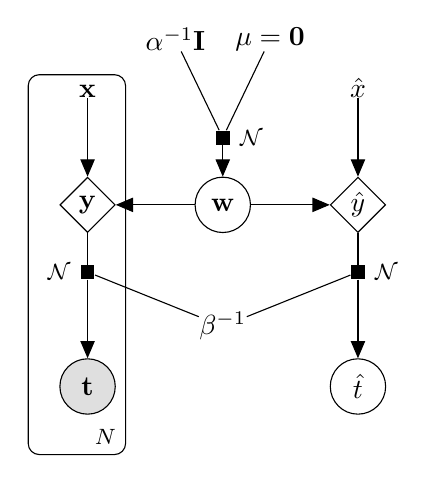
\begin{tikzpicture}

      % Define nodes
	  \node[const]                             (x) {$\mathbf{x}$};
	  \node[det, below=of x]                   (y) {$\mathbf{y}$};
	  \node[latent, right=of y]                (w) {$\mathbf{w}$};
	  \node[const, below=of w]                 (beta) {$\beta^{-1}$};
	  \node[det, right=of w]                   (y-hat) {$\hat{y}$};
	  \node[const, above=of y-hat]             (x-hat) {$\hat{x}$};
	  \factor[above=of w]{w-f}{right:$\mathcal{N}$}{}{};
	  \node[const, above=of w-f, xshift=.6cm]  (mu) {$\mathbf{\mu}=\mathbf{0}$};
	  \node[const, above=of w-f, xshift=-.6cm]   (alpha) {$\mathbf{\alpha}^{-1}\mathbf{I}$};
	  \factor[below=of y]{t-f}{left:$\mathcal{N}$}{}{};
	  \factor[below=of y-hat]{hat-f}{right:$\mathcal{N}$}{}{};
	  \node[obs, below=of t-f]                   (t) {$\mathbf{t}$};
	  \node[latent, below=of hat-f]                 (t-hat) {$\hat{t}$};

	  % Connect the nodes
	  \edge {x,w} {y} ; 
	  \edge {x-hat,w} {y-hat} ; 
	  \factoredge{mu, alpha}{w-f}{w}
	  \factoredge{y,beta}{t-f}{t}
	  \factoredge{y-hat,beta}{hat-f}{t-hat}

	  % Plates
	  \plate {xt} {(x)(y)(t-f)(t-f-caption)(t)(y.east)} {$N$} ;

	\end{tikzpicture}

  \end{center}
  \caption{Curve fitting model in PRML \$1.2.5}
\end{figure}

\end{document}

